\documentclass[12pt]{article}
\usepackage[margin=0.8in]{geometry}
\usepackage{amsmath}
\usepackage{hyperref}
\usepackage{graphicx}
\usepackage{float}
\usepackage{caption}
\usepackage{subcaption}

\title{Numerical analysis: Assignment 7}
\author{Niccolo Zuppichini}
\begin{document}

\maketitle
\section*{Exercise 1}

Using the taylor expansion we can write the following identities: 
%TODO check if it s O(3)

\begin{equation}
\begin{split}
u(x-2h) = u(x) -2 h u'(x) + \frac{4 h^2}{2} u''(x) - \frac{ (2h)^3}{3!} u'' + O(h^4) \\
u(x+h) = u(x) + h u'(x) + \frac{h^2}{2} u''(x) + \frac{h^3}{3!} u'' + O(h^4) \\
u(x+2h) = u(x) + 2 h u'(x) + \frac{4 h^2}{2} u''(x) + \frac{ (2h)^3}{3!} u'' + O(h^4)  \\
\end{split}	
\label{eq:taylor}
\end{equation}

Then we can express the problem of finding the coefficients a,b,c,d,e for the third order finite difference as follows: 
\begin{equation}
\centering
  \begin{split}
    a u(x-2h) + b u(x) + c u(x+h) + d u(x+2h) =  \\
    (a+b+c+d) u(x) + (-a2h +ch +d 2h) u'(x) + \\
    (a \frac{(2h^2)}{2} + c \frac{h^2}{2} + d \frac{(2h^2)}{2}) u''(x) +
     ( -\frac{(2h)^3}{3!} a +\frac{h^3}{3!} c + \frac{(2h)^3}{3!} d) u''(x)
  \end{split}
\end{equation}


We know want to compute these coefficients to obtain a finite difference in function of $u(x-2h), u(x+h), u(x), u(x+h), u(x+2h)$. This is translated into solving a system of equations: 

\begin{equation}
	\begin{cases}
		a+ b + c + d = 0  \\
		-2h a +h c + 2h d = 1 \\
		(2h)^2 a + h^2 c + (2h)^2 d = 0 \\
		-(2h)^3 a +h^3c + (2h)^3d  = 0 \\
	\end{cases}
	\label{eq:system}
\end{equation}


The system of equations can be solve as a linear system $Ax=b$. Moreover, by equation \ref{eq:system}, $A$ is a transposed Vandermonde matrix multiplied by $\frac{1}{h^d}$. The vector $b$ on the other hand is given by $b[d] = d!$ where $d$ is the derivative you want to approximate (in Eq. \ref{eq:system} $d=1$). Also, note, that $n>d$ where $n$ is the number of sample points. Following these indications, I've implemented it in \textit{computation.py} resulting in the following third order non centered finite difference method:\\

\begin{equation}
	u'(x) \approx \frac{-0.8\bar{3} u(x-2h) -u(x) + 1.\bar{3} u(x+h) - 0.25 u(x+2h)}{h}
	\label{eq:solution} + O(h^3)
\end{equation}

The leading error $O(h^3)$ is given by dividing the error given by expressing each component as a taylor expansion (Eq. \ref{eq:taylor}) by $h$ to express the first derivative $u'(x)$. 

Then I've evaluated the function in the assignment at the point 1 for different values of $h$ as asked in the assignment (Figure \ref{fig:error}). For $k=15$ the $h$ value is too near machine error $\epsilon$ and the accuracy deteriorates. The best values of $h$ are, as predicted by the theory, for $\sqrt{\epsilon}$.  The code can be found in \textit{main.py}. \\


\begin{figure}[H]
\centering
	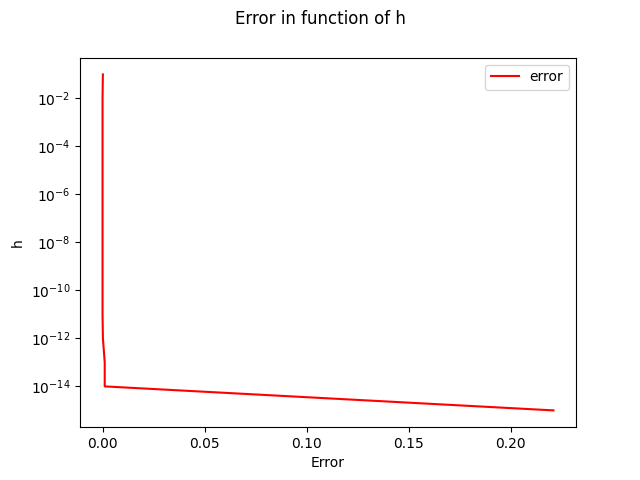
\includegraphics[width = 0.8\columnwidth]{error_plot.png}
	\caption{}
	\label{fig:error}
\end{figure}

\end{document}